\documentclass[a4paper,11pt]{article}
\pdfoutput=1 % if your are submitting a pdflatex (i.e. if you have
             % images in pdf, png or jpg format)

\usepackage{jinstpub} % for details on the use of the package, please
                      % see the JINST-author-manual

\usepackage{lineno}
\linenumbers

\title{Development of a high bandwidth readout chain for the CMS Phase-2 pixel upgrade}

%% %simple case: multiple authors, same institution
\author{C. Smith}
\affiliation{The University of Kansas,\\Lawrence, Kansas 66045, USA}

% \affiliation{The University of Kansas\\1251 Wescoe Hall Dr.\\Lawrence, KS 66045, United States}

% From CMS publication:
% The University of Kansas, Lawrence, Kansas 66045, USA
% From KU physics website:
% The University of Kansas, 1251 Wescoe Hall Dr. Lawrence, KS 66045, United States

% more complex case: 4 authors, 3 institutions, 2 footnotes
% \author[a,b,1]{F. Irst,\note{Corresponding author.}}
% \author[c]{S. Econd,}
% \author[a,2]{T. Hird\note{Also at Some University.}}
% \author[c,2]{and Fourth}

% The "\note" macro will give a warning: "Ignoring empty anchor..."
% you can safely ignore it.

% \affiliation[a]{One University,\\some-street, Country}
% \affiliation[b]{Another University,\\different-address, Country}
% \affiliation[c]{A School for Advanced Studies,\\some-location, Country}

% e-mail addresses: only for the corresponding author
\emailAdd{caleb.smith@ku.edu}

\abstract{
The CMS collaboration is building a new inner tracking pixel detector for the High-Luminosity LHC.
Each pixel readout chip will be controlled with a single serial input stream at 160 Mbps and will send out data via four CML 1.28 Gbps outputs.
The readout chips will be grouped in modules and connected with up to 1.6 m long low-mass electrical links to the low power gigabit transceivers (lpGBT) and versatile transceivers (VTRx+) that send the data optically to off-detector electronics at 10 Gbps.
The development and the characterization of these components is presented along with system tests of the readout chain.
}

\keywords{Only keywords from JINST's keywords list please}

% \arxivnumber{1234.56789} % only if you have one

% \collaboration{\includegraphics[height=17mm]{example-image}\\[6pt]
%   XXX collaboration}
% or
\collaboration[c]{on behalf of the CMS collaboration}


% if you write for a special issue this may be useful
\proceeding{Topical Workshop on Electronics for Particle Physics\\
  September 20--24, 2021\\
  Online event}

\begin{document}
\maketitle
\flushbottom

% Comment on abbreviations
% We suggest not to abbreviate: ``section'', ``appendix'', ``figure''
% and ``table'', but ``eq.'' and ``ref.'' are welcome. Also, please do
% not use \texttt{\textbackslash emph} or \texttt{\textbackslash it} for
% latin abbreviaitons: i.e., et al., e.g., vs., etc.

\section{Readout Chain}
\label{sec:readout}

Readout chain section.

\section{Electrical Links}
\label{sec:electrical}

Electrical links section.

\subsection{Crosstalk Measurements}

Crosstalk measurements section.

\begin{figure}[htbp]
\centering
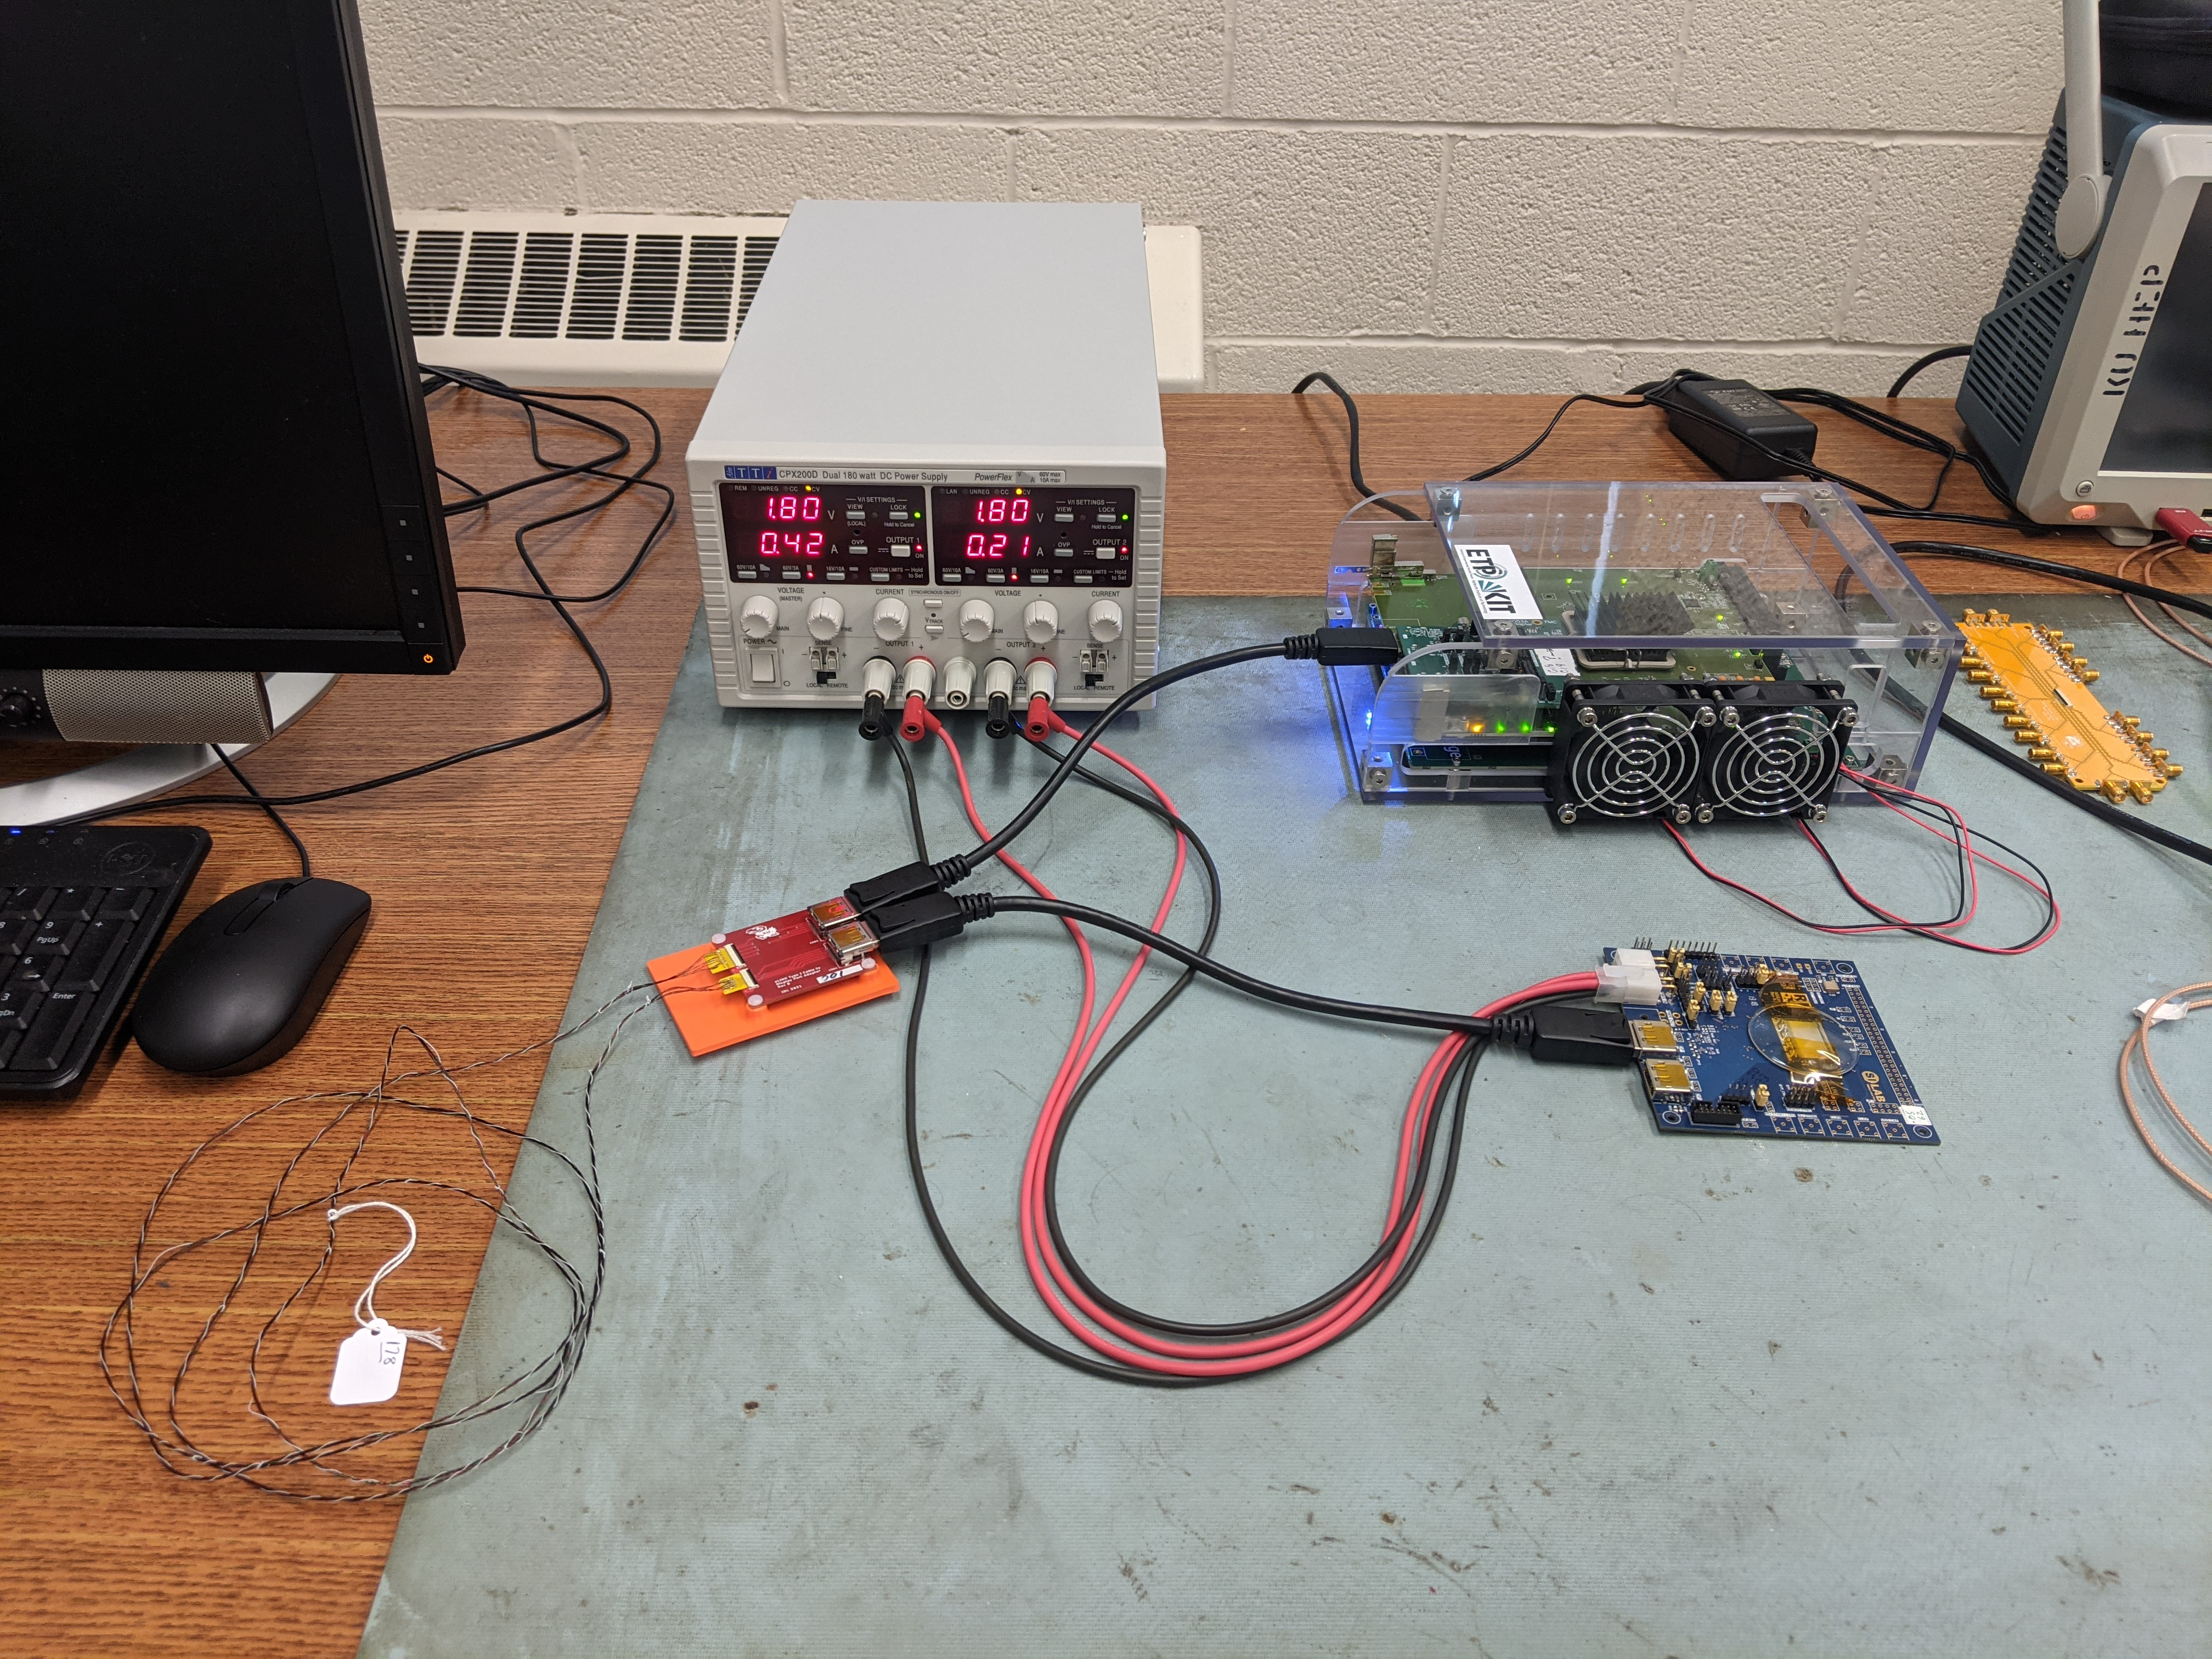
\includegraphics[width=0.5\textwidth,origin=c]{../figures/fc7_elink_scc_setup.jpg}
\qquad
\includegraphics[width=0.4\textwidth,origin=c]{../figures/BERT_TAP0_vs_Length.pdf}
\caption{
\label{fig:tap0_vs_length}
Measurement of signal amplitude (set by TAP0) for electrical links as a function of e-link length for 34 and 36 AWG e-links.
In the hardware setup (left), an FC7 is connected to an SCC through two commercial DP cables, an adapter board, and an e-link for control and readout communication of an RD53A chip.
The measurements (right) show the TAP0 setting to achieve a bit error rate of $10^{-11}$ errors per second for e-links of different lengths.
% For e-links of different lengths, the TAP0 setting to achieve a bit error rate of $10^{-11}$ errors per second is measured (right).
The necessary signal amplitude increases with e-link length as expected.
Good performance is seen for e-links up to 2.0 meters.
}
\end{figure}

\begin{figure}[htbp]
\centering
\includegraphics[width=0.5\textwidth,origin=c,angle=270]{../figures/external_crosstalk_setup.jpg}
\qquad
\includegraphics[width=0.5\textwidth,origin=c]{../figures/BERT_TAP0_Scan_External_Crosstalk.pdf}
\caption{
\label{fig:external_crosstalk}
Measurement of the effect of external crosstalk on data transmission.
Two e-links (1.4 meters, 36 AWG) are twisted together (left), with a victim e-link connected between an FC7 and SCC to readout from an RD53A chip, and an aggressor e-link connected to a KC705.
The KC705 sends PRBS signals on four e-link channels on the aggressor at different amplitudes.
To mitigate the effect of external crosstalk from a large aggressor amplitude, the victim amplitude set by TAP0 only requires a small increase.
Thus, external crosstalk from the single aggressor e-link has a small effect on readout over the victim e-link.
% Thus, the effect of external crosstalk from a single aggressor e-link is small.
}
\end{figure}

\section{Optical Links}
\label{sec:optical}

Optical links seciton.

\begin{figure}[htbp]
\centering
\includegraphics[width=0.8\textwidth,origin=c]{../figures/lpGBT_eye.pdf}
\caption{
\label{fig:lpgbt_eye}
Eye opening monitor from an lpGBT for the 2.56 Gbps optical down link.
The plot shows the height of the eye as a function of sampling phase.
The high-speed input to the lpGBT is compared to a variable (5-bit), fixed voltage by a comparator sampled with a phase interpolated clock.
Transitions of the comparator are counted; within the eye the output should toggle, above or below no transitions are expected.
The color scale shows the number of transitions.
The region with high toggle count corresponds to the eye opening.
Equalization parameters are at default settings.
}
\end{figure}

\begin{figure}[htbp]
\centering
\includegraphics[width=1.0\textwidth,origin=c]{../figures/lpGBT_bert.png}
\caption{
\label{fig:lpgbt_bert}
Scan of bit-error rate vs. clock sampling phase and equalization setting for e-port receivers on the lpGBT driven by the RD53A pixel readout chip over commercial DP cable, adapter and Molex FPC cables.
The source is a PRBS7 generator in the RD53A read out chip, compared to the internal error checker in the lpGBT.
Points in green have zero observed errors and report the reciprocal of the number of bits checked.
The phase at the eye crossing is clearly seen.
Equalization settings affect the timing slightly.
}
\end{figure}

% Appendices

\appendix
\section{Example appendix title}

Here is this appendix.

\acknowledgments

Put acknowledgments here.

% We suggest to always provide author, title and journal data:
% in short all the informations that clearly identify a document.

\begin{thebibliography}{99}

\bibitem{a}
Author, \emph{Example Title},
arxiv:1234.5678.

% \bibitem{a}
% Author, \emph{Title}, \emph{J. Abbrev.} {\bf vol} (year) pg.
%
% \bibitem{b}
% Author, \emph{Title},
% arxiv:1234.5678.
%
% \bibitem{c}
% Author, \emph{Title},
% Publisher (year).

% Please avoid comments such as "For a review'', "For some examples",
% "and references therein" or move them in the text. In general,
% please leave only references in the bibliography and move all
% accessory text in footnotes.

% Also, please have only one work for each \bibitem.

\end{thebibliography}
\end{document}
